\chapter{Datacenter network model} \label{model}

In this chapter I describe common models of networks and data-centers as well as describe the model I implemented.

\section{Datacenter background} \label{model-dc}

\subsection{Network configuration} \label{model-network}

% A lot of this section is a mess
Most datacenters \rotornet\cite{handley_re-architecting_2017}\opera
There are anywhere from 5 to 50 servers in a rack, each connected to a switch typically at the top, giving it the common name "Top of Rack switch" or ToR.
A "small" datacenter may have around 5,000 machines, large ones up to 250,000 or more. % TODO citation?

The racks themselves are connected together through different fabrics, and switch technologies.
The topology and technologies behind these is extremely varied \cite{kassing_beyond_2017}, and the subject of extensive research \opera\rotornet (TODO Xpander). % TODO cite

CLOS networks, or fat-trees, are a common topology in data-centers today \cite{singh_jupiter_2015}\cite{noauthor_reinventing_2019}\cite{noauthor_introducing_2014}.
They consist of a hierarchy of switches, with their bandwidth equally split up and down the hierarchy.
For cost-reduction purposes, it is common to have the first layer, from the servers to the ToR switch to be oversubscribed: the servers are able to send more traffic than the rack can handle.

\begin{figure}[h]
    \centering
    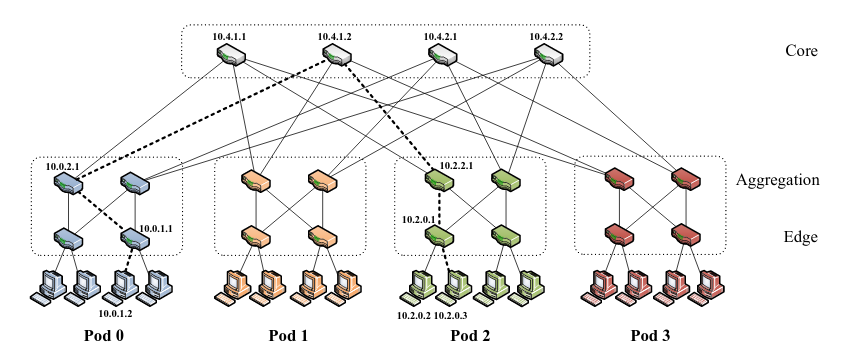
\includegraphics[width=\textwidth]{fat-tree}
    \label{fig:fat-tree}
    \caption{An example of a fat-tree topology from \cite{al-fares_scalable_2008}}
\end{figure}

The typical bandwidth vary but are in the 10Gbps to 100Gbps scale for these links.
Some networks assume different link speeds between the ToRs than from server to ToR, others are uniform.

The latencies involved are often extremely small, on the order of tens of nanoseconds.


\subsection{Traffic modelling} \label{model-traffic}

There are a few well studied datacenter traffic models (datamining, websearch, Chen Stefan Manya paper, more), with a common takeaway being that datacenter traffic is hard to predict.

Traffic distribution can be broken down into multiple dimensions: overall load, skeweness, and flow size distribution.


Overall load corresponds to how much traffic is being offered onto the network relative to how much capacity the network has.
It is important to note that this does not mean that the network is able to 100\% load, most networks are overwhelmed far before.
The reason for this is simple: if on average, it takes 4 hops to get to the destination, traffic is essentially being sent 4 times, making any load above 25\% impossible to satisfy.

The traffic may be fairly uniform, each sender and receiver being involved in traffic all around the datacenter, or very concentrated, with a few "hot" racks being very active with each other, the rest of the datacenter quiet.
Describing these patterns can become quite complex, as there may be multiple "hot" regions mostly not interacting with each other.
Throughput this thesis, and in most of the literature, we tend to be concerned about uniform traffic.

Finally, the flow size distribution corresponds to how big each flow is expected to be \cite{alizadeh_data_2010}.
Some workloads, such as websearch, consists mostly of many small flows.
Others, such as datamining, are comparatively much bigger.
Machine working loads also typically create a large demand, for example in a ring, using all the networking resources available.

\section{Simulation Model} \label{model-sim}

The datacenter model used by Rustasim was chosen to emulate closely that of Opera, to allow for comparison and verification of the results.

The model used in Rustasim \ref{rustasim}, consists of two actor types: routers and servers, and three model-level event types: \code{packet}, \code{flow} and \code{timeout} events.
The servers are organized in racks, themselves interconnected through a user-chosen topology.

A \code{packet} event carries with it the corresponding packet and signals the arrival of that packet to the actor who then forwards it along appropriately.
If the packet carried by the event arrives at its destination, it is acked.
If the packet is an ack arriving back at the sender, the flow reacts appropriately.\\

\code{Flow} events are received directly by servers and indicate the start of a new flow at that server.
\code{Timeouts} are received by the senders themselves and may cause a packet to be retransmitted if it hasn't been acknowledged.

Following with Opera's design, the queue sizes are TODO, the link speeds are all 10Gbps.
The latencies in the Opera simulator are set to 0 from server to ToR, and 500ns from ToR to ToR.
Unfortunately, conservative scheduling algorithms are unable to make progress with 0 latency, so I've set all latencies to be 500ns.
This has a measurable impact on the completion time of very small flows, where latency is the main contributor, but otherwise does not impact the results.
This is discussed more in section \ref{replication}.


\subsection{TCP} \label{model-tcp}

In this model, a limited version of TCP is implemented with a fixed congestion window of size 30, similar to choices Opera makes.
Although it is possible to implement a more realistic version of TCP, this simple version is close to the Opera simulator that the results check out.
